\documentclass[12pt]{article}

\usepackage[right=1in, top=1in, left=1in, bottom=1in]{geometry}
\usepackage[parfill]{parskip}
\usepackage{hyperref, float}
\hypersetup{
    colorlinks=true,
    linkcolor=blue,
    filecolor=magenta,      
    urlcolor=cyan,
}

\usepackage{simpleoptics}


\begin{document}


\begin{titlepage}
\vspace*{\fill}
\begin{center}
{\Huge Simple Optics Documentation}\\[0.5cm]
{\Large Version: 1.1.1}\\[0.4cm]
{\Large Date: $7^{th}$ of September 2019}\\[0.2cm]
{\small Author: Justin Cawood}
\end{center}
\vspace*{\fill}
\end{titlepage}

\newpage

\tableofcontents

\newpage

\section{Important Info}

All optics diagrams drawn with this package \textbf{must} be contained within a "tikzpicture" environment

Example.

$\backslash$begin\{center\}

$\backslash$begin\{tikzpicture\}

$\backslash$mirror\{0\}\{0\}\{-4\}\{3\}

$\backslash$end\{tikzpicture\}

$\backslash$end\{center\}

\begin{figure}[H]

\begin{center}

\begin{tikzpicture}

\mirror{0}{0}{-4}{3}

\end{tikzpicture}

\end{center}

\caption{Simple mirror example}
\end{figure}

\section{Quick Macro Reference}

The available macros are

\begin{itemize}
\item $\backslash$mirror\{x\}\{y\}\{focal length\}\{mirror height\}
\item $\backslash$leftplanoconvexlens\{x\}\{y\}\{focal length\}\{mirror height\}\{thickness\}
\item $\backslash$rightplanoconvexlens\{x\}\{y\}\{focal length\}\{mirror height\}\{thickness\}
\item $\backslash$leftplanoconcavelens\{x\}\{y\}\{focal length\}\{mirror height\}\{thickness\}
\item $\backslash$rightplanoconcavelens\{x\}\{y\}\{focal length\}\{mirror height\}\{thickness\}
\item $\backslash$biconvexlens\{x\}\{y\}\{focal length\}\{mirror height\}\{thickness\}
\item $\backslash$biconcavelens\{x\}\{y\}\{focal length\}\{mirror height\}\{thickness\}
\item $\backslash$convexconcavelens\{x\}\{y\}\{focal length\}\{mirror height\}\{thickness\}
\item $\backslash$concaveconvexlens\{x\}\{y\}\{focal length\}\{mirror height\}\{thickness\}
\end{itemize}


\section{Mirrors}

Mirrors can be drawn using the $\backslash$mirror macro.

The macro takes the following parameters, all of which are required.

$\backslash$mirror\{x\}\{y\}\{focal length\}\{mirror height\}

The parameters x and y are the coordinates for where the mirror will be placed. The focal length and height are simply the focal length and height of the mirror.

If you want to flip the mirror the other way, just specify a negative focal length. Examples of both are done below with the code below each.


\begin{minipage}{\textwidth}
\begin{minipage}{0.5\textwidth}

\begin{figure}[H]

\begin{center}

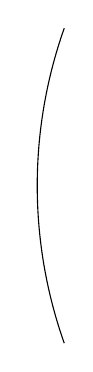
\begin{tikzpicture}

\mirror{0}{0}{3}{2}

\end{tikzpicture}

\end{center}

\caption{Positive focal length example}
\end{figure}

$\backslash$begin\{center\}

$\backslash$begin\{tikzpicture\}

$\backslash$mirror\{0\}\{0\}\{3\}\{4\}

$\backslash$end\{tikzpicture\}

$\backslash$end\{center\}
\end{minipage}
\begin{minipage}{0.5\textwidth}

\begin{figure}[H]

\begin{center}

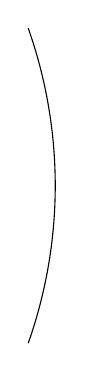
\begin{tikzpicture}

\mirror{0}{0}{-3}{2}

\end{tikzpicture}

\end{center}

\caption{Negative focal length example}
\end{figure}

$\backslash$begin\{center\}

$\backslash$begin\{tikzpicture\}

$\backslash$mirror\{0\}\{0\}\{-3\}\{4\}

$\backslash$end\{tikzpicture\}

$\backslash$end\{center\}
\end{minipage}
\end{minipage}

\section{Lenses}

The lenses are made using mirrors.

There are a few different lenses that can be drawn with this package, each of which has its own macro.

\subsection{Plano Lenses}
Plano lenses have one flat side and the other side is either convex or concave.

The plano lenses have macros following this format

$\backslash$leftplano"convex/concave"lens\{x\}\{y\}\{focal length\}\{mirror height\}\{thickness\}

or

$\backslash$rightplano"convex/concave"lens\{x\}\{y\}\{focal length\}\{mirror height\}\{thickness\}

\subsubsection{Plano-Convex Lenses}

This package provides two plano-covex lens macros. One faces left and the other right. The left and right refer to the flat side of the lens. These are shown below.

\begin{minipage}{\textwidth}
\begin{minipage}{0.5\textwidth}

\begin{figure}[H]

\begin{center}

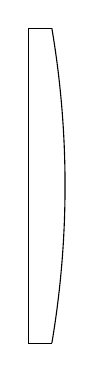
\begin{tikzpicture}

\leftplanoconvexlens{0}{0}{3}{2}{0.3}

\end{tikzpicture}

\end{center}

\caption{Left plano convex lens}
\end{figure}

$\backslash$begin\{center\}

$\backslash$begin\{tikzpicture\}

$\backslash$leftplanoconvexlens\{0\}\{0\}\{3\}\{4\}\{0.3\}

$\backslash$end\{tikzpicture\}

$\backslash$end\{center\}
\end{minipage}
\begin{minipage}{0.5\textwidth}

\begin{figure}[H]

\begin{center}

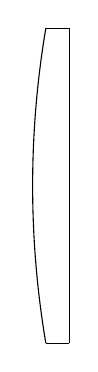
\begin{tikzpicture}

\rightplanoconvexlens{0}{0}{3}{2}{0.3}

\end{tikzpicture}

\end{center}

\caption{Right plano convex lens}
\end{figure}

$\backslash$begin\{center\}

$\backslash$begin\{tikzpicture\}

$\backslash$rightplanoconvexlens\{0\}\{0\}\{3\}\{4\}\{0.3\}

$\backslash$end\{tikzpicture\}

$\backslash$end\{center\}
\end{minipage}
\end{minipage}

\subsubsection{Plano-Concave Lenses}

The same can be done with plano concave lenses. Again there are two available macros. One faces left and the other right. The left and right refer to the flat side of the lens. These are shown below.

\begin{minipage}{\textwidth}
\begin{minipage}{0.5\textwidth}

\begin{figure}[H]

\begin{center}

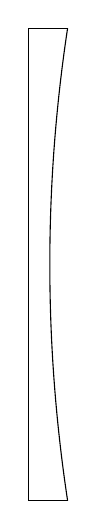
\begin{tikzpicture}

\leftplanoconcavelens{0}{0}{5}{3}{0.5}

\end{tikzpicture}

\end{center}

\caption{Left plano concave lens}
\end{figure}

$\backslash$begin\{center\}

$\backslash$begin\{tikzpicture\}

$\backslash$leftplanoconcavelens\{0\}\{0\}\{5\}\{3\}\{0.5\}

$\backslash$end\{tikzpicture\}

$\backslash$end\{center\}
\end{minipage}
\begin{minipage}{0.5\textwidth}

\begin{figure}[H]

\begin{center}

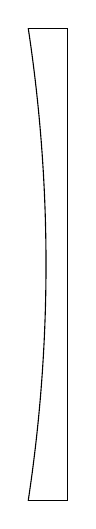
\begin{tikzpicture}

\rightplanoconcavelens{0}{0}{5}{3}{0.5}

\end{tikzpicture}

\end{center}

\caption{Right plano concave lens}
\end{figure}

$\backslash$begin\{center\}

$\backslash$begin\{tikzpicture\}

$\backslash$rightplanoconcavelens\{0\}\{0\}\{5\}\{3\}\{0.5\}

$\backslash$end\{tikzpicture\}

$\backslash$end\{center\}
\end{minipage}
\end{minipage}

\subsection{Bi Lenses}

Bi lenses are made of two mirrors facing opposite directions.

Bi lenses have macros with this format 

$\backslash$bi"convex/concave"lens\{x\}\{y\}\{focal length\}\{mirror height\}\{thickness\}

\subsubsection{Bi-Convex Lens}

\begin{figure}[H]

\begin{center}

\begin{tikzpicture}

\biconvexlens{0}{0}{1}{2}{1}

\end{tikzpicture}

\end{center}

\caption{Bi convex lens}
\end{figure}

$\backslash$begin\{center\}

$\backslash$begin\{tikzpicture\}

$\backslash$biconvexlens\{0\}\{0\}\{1\}\{2\}\{1\}

$\backslash$end\{tikzpicture\}

$\backslash$end\{center\}

\subsubsection{Bi-Concave Lens}

\begin{figure}[H]

\begin{center}

\begin{tikzpicture}

\biconcavelens{0}{0}{1}{3}{5}

\end{tikzpicture}

\end{center}

\caption{Bi concave lens}
\end{figure}

$\backslash$begin\{center\}

$\backslash$begin\{tikzpicture\}

$\backslash$biconcavelens\{0\}\{0\}\{1\}\{3\}\{5\}

$\backslash$end\{tikzpicture\}

$\backslash$end\{center\}

\subsection{Convex-Concave and Concave-Convex Lenses}

Convex and concave mirrors can be combined to make convex-concave lenses and concave-convex lenses.

They have macros with the format

$\backslash$convexconcavelens\{x\}\{y\}\{focal length\}\{mirror height\}\{thickness\}

$\backslash$concaveconvexlens\{x\}\{y\}\{focal length\}\{mirror height\}\{thickness\}

\begin{minipage}{\textwidth}
\begin{minipage}{0.5\textwidth}

\begin{figure}[H]

\begin{center}

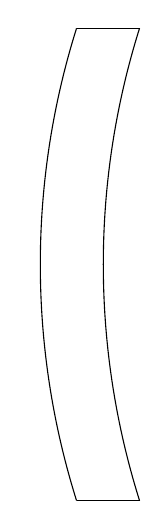
\begin{tikzpicture}

\convexconcavelens{0}{0}{2.5}{3}{0.8}

\end{tikzpicture}

\end{center}

\caption{Convex-Concave lens}
\end{figure}

$\backslash$begin\{center\}

$\backslash$begin\{tikzpicture\}

$\backslash$convexconcavelens\{0\}\{0\}\{2.5\}\{3\}\{0.8\}

$\backslash$end\{tikzpicture\}

$\backslash$end\{center\}
\end{minipage}
\begin{minipage}{0.5\textwidth}

\begin{figure}[H]

\begin{center}

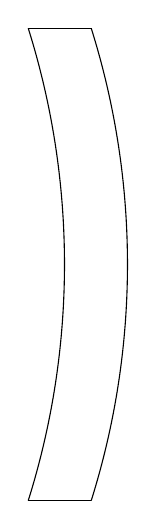
\begin{tikzpicture}

\concaveconvexlens{0}{0}{2.5}{3}{0.8}

\end{tikzpicture}

\end{center}

\caption{Concave-Convex lens}
\end{figure}

$\backslash$begin\{center\}

$\backslash$begin\{tikzpicture\}

$\backslash$concaveconvexlens\{0\}\{0\}\{2.5\}\{3\}\{0.8\}

$\backslash$end\{tikzpicture\}

$\backslash$end\{center\}
\end{minipage}
\end{minipage}

\section{Multiple At Once}

The macros can all be used at the same time to produce diagrams with multiple lenses and/or mirrors.


\begin{figure}[H]

\begin{center}

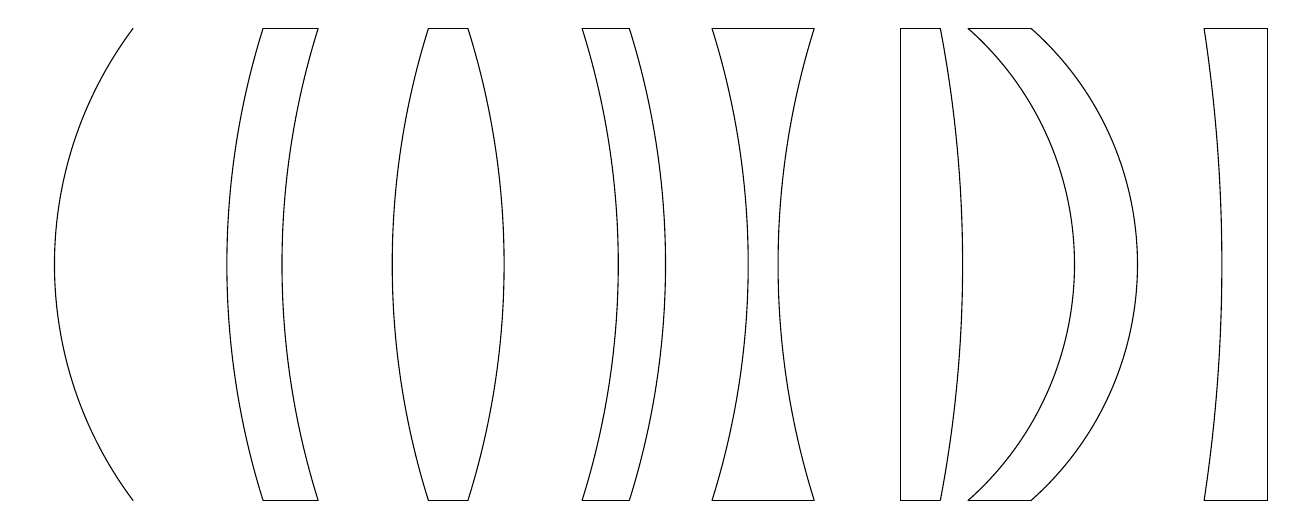
\begin{tikzpicture}

\mirror{1}{0}{2.5}{3}
\convexconcavelens{3}{0}{2.5}{3}{0.7}
\biconvexlens{5}{0}{2.5}{3}{0.5}
\concaveconvexlens{7}{0}{2.5}{3}{0.6}
\biconcavelens{9}{0}{2.5}{3}{1.3}
\leftplanoconvexlens{11}{0}{4}{3}{0.5}
\concaveconvexlens{12}{0}{1}{3}{0.8}
\rightplanoconcavelens{15}{0}{5}{3}{0.8}

\end{tikzpicture}

\end{center}

\caption{Concave-Convex lens}
\end{figure}

$\backslash$begin\{center\}

$\backslash$begin\{tikzpicture\}

$\backslash$mirror\{1\}\{0\}\{2.5\}\{3\}

$\backslash$convexconcavelens\{3\}\{0\}\{2.5\}\{3\}\{0.7\}

$\backslash$biconvexlens\{5\}\{0\}\{2.5\}\{3\}\{0.5\}

$\backslash$concaveconvexlens\{7\}\{0\}\{2.5\}\{3\}\{0.6\}

$\backslash$biconcavelens\{9\}\{0\}\{2.5\}\{3\}\{1.3\}

$\backslash$leftplanoconvexlens\{11\}\{0\}\{4\}\{3\}\{0.5\}

$\backslash$concaveconvexlens\{12\}\{0\}\{1\}\{3\}\{0.8\}

$\backslash$rightplanoconcavelens\{15\}\{0\}\{5\}\{3\}\{0.8\}

$\backslash$end\{tikzpicture\}

$\backslash$end\{center\}


\end{document}